\newpage
\chapter{Speech Signal Processing}
\label{chapter:speech-processing}

\section{Analog-to-Digital Conversion}
Voices in real life are analog signals, hence before conducting digital signal processing techniques, analog-to-digital conversions are required.\\

Given a continuous-time signal $s(t)$, we define the \textit{sampled signal} by
\begin{equation}
s[n] = s(nT_s) = s(\frac{n}{F_s})
\end{equation}
where $T_s$ is the sampling interval and $F_s$ is the sampling rate.\\

$T_s$ should be carefully chosen in order to avoid distortion caused by aliasing. Telephony since the 1950s limits the information bandwidth to 300-3400 Hz \cite{EVW-report}. However, in normal conversational speech, the frequency content is mainly between 0-8000 Hz \cite{uysal2005bandwidth}. According to Nyquist-Shannon sampling theorem, we set the folding frequency $\frac{F_s}{2}$ = 8000 Hz, i.e. $F_s$ = 16 kHz.

%--------------------------------------------
%--------------------------------------------

\section{Pre-emphasis}

The speech production system inherently attenuates speech signal by a negative spectral slope per decade. In addition, human hearing is more sensitive to frequency band above 1 kHz \cite{picone1993signal}. However, as is depicted in Fig. \ref{zero_fft}, frequency components below 1 kHz predominantly comprise the spectrum. Hence, it is advantageous to employ a high-pass filter to amplify the high frequency range.\\

A first-order FIR filter represented by (\ref{high-pass-filter}) is widely implemented, including the previous group where $\alpha = 0.95$ \cite{EVW-report}. The merits of this FIR filter include simplicity and efficiency. However, Fig. \ref{pre_emphasis_filter} (\textcolor{orange_matlab}{orange} dash-dot line) shows that frequencies below 500 Hz are severely suppressed even though frequencies above 3 kHz are successfully amplified. Considering the potential interference caused by high-frequency noise, attenuating low frequencies too much will result in the decline of signal-to-noise ratio (SNR).

\begin{equation}
\label{high-pass-filter}
y[n] = x[n] - \alpha x[n-1]
\end{equation}

\begin{figure}[H]
\begin{minipage}[t]{0.5\linewidth}
\centering
\minipageplot{ang/pre_emphasis_filter}
\caption{Pre-emphasis Filters}
\label{pre_emphasis_filter}
\end{minipage}
\begin{minipage}[t]{0.5\linewidth}
\centering
\minipageplot{ang/zero_fft}
\caption{Spectra of Word \textit{zero}}
\label{zero_fft}
\end{minipage}
\end{figure}

Suggested by Professor Erik \textsc{Weyer}, we try to devise a second-order \textit{shelving filter} widely utilized in audio equalization to pre-emphasize the speech signal. With the aid of \cite{DAFX_book}, setting center frequency of transition band $F_c$ = 1000 Hz and gain $G$ = 6 dB, eventually we obtain an appropriate filter that effectively amplifies high-frequency components without attenuating low frequencies. Fig. \ref{pre_emphasis_filter} (\textcolor{navy_matlab}{navy} solid line) shows the frequency response of this shelving filter and Fig. \ref{zero_fft} shows the spectrum and pre-emphasized spectrum of word \textit{zero}.\\

The pre-emphasis filter is mathematically represented by (\ref{shelving-filter}) and (\ref{shleving-coef}). Equations for calculating filter coefficients are available in the Appendix on page \pageref{shelving-appendix}.

\begin{equation}
\label{shelving-filter}
y[n] = \frac{1}{a_0} \Big( b_0 x[n] + b_1 x[n-1] + b_2 x[n-3] - a_1 y[n-1] - a_2 y[n-2] \Big)
\end{equation}
where
\begin{align}
\label{shleving-coef}
&\begin{cases}
a_0 = 1\\
a_1 = -1.523796\\
a_2 = 0.649345
\end{cases}
&\begin{cases}
b_0 = 1.861856\\
b_1 = -3.102851\\
b_2 = 1.366544
\end{cases}
\end{align}

%--------------------------------------------
%--------------------------------------------

\section{Framing \& Windowing}

Speech signals are time-varying signals, but due to the inertial motion of articulators (speech organs such as the tongue, lips and palate), speech can be considered statistically stationary in a short-time period (approximately 30 ms) \cite{brandstein1995practical}. The time period of 30 ms indicates 30 ms $\times$ 16000 Hz = 480 samples per frame. We take $N = 512$ to achieve a power of 2 in order that Fast Fourier Transform can be effectively conducted during the following \textit{power spectrum} procedure in \fullref{subsection:mfcc}.\\

The framing operation can be finished by multiplying the signal by a moving window. For the $j$-th frame and frame length $N$, mathematical equation is given in (\ref{eq:windowing}).

\begin{equation}
\label{eq:windowing}
s_j[n] =
\begin{cases}
w[n] s[n+jN] & n = 1, 2, \dots, N\\
0 & \text{otherwise}
\end{cases}
\end{equation}

The simplest and easiest-to-implement window is a rectangular window represented by (\ref{eq:rectagular-window}).
\begin{equation}
\label{eq:rectagular-window}
w[n] =
\begin{cases}
1, & n = 1, 2, \dots, N\\
0, & \text{otherwise}
\end{cases}
\end{equation}

However, the selection of a proper window always involves a trade-off between high \textbf{frequency resolution} and low \textbf{spectral leakage}. On the one hand, convolution with mainlobe smooths the estimate over nearby frequencies and the frequency resolution is determined by the width of the mainlobe. On the other hand, the sidelobes cause sidelobe energy to appear in the spectrum, i.e. spectral leakage. (from ELEN90058 \textit{Signal Processing} lecture slides by Erik \textsc{Weyer})

\begin{figure}[H]
\begin{minipage}[t]{0.5\linewidth}
\centering
\minipageplot{ang/windows_time}
\caption{Windows in Time Domain}
\label{windows_time}
\end{minipage}
\begin{minipage}[t]{0.5\linewidth}
\centering
\minipageplot{ang/windows_frequency}
\caption{Windows in Frequency Domain}
\label{windows_frequency}
\end{minipage}
\end{figure}

\begin{table}[H]
\caption{Windows Properties for $N = 16$}
\label{table:windows}
\begin{tabu} to \textwidth {XXXXX}
\toprule
Windows &Rectangular &Hanning &Hamming &Blackman\\
\hline
Mainlobe width &$0.125 \pi$ &$0.2353 \pi$ &$0.2985 \pi$ &$0.4 \pi$\\
\hline
Peak sidelobe &-13.2 dB &-31.5 dB &-39.8 dB &-58.6 dB\\
\bottomrule
\end{tabu}
\end{table}

In terms of the windows involved in Fig. \ref{windows_time}, Fig. \ref{windows_frequency} and Table \ref{table:windows}, \textit{rectangular} window has the best frequency resolution (narrowest mainlobe) at the expense of highest spectral leakage (biggest sidelode peak) while \textit{Blackman} window has the lowest spectral leakage (smallest sidelode peak) accompanied by worst frequency resolution (widest mainlobe). Eventually, we choose an intermediate \textit{Hamming} window given in (\ref{eq:hamming}).

\begin{equation}
\label{eq:hamming}
w[n] = \alpha - \beta \cos \left( \frac{2 \pi n}{N-1} \right) \quad n = 1, 2, \dots, N
\end{equation}
where $\alpha = 25/46 \approx 0.54$ and $\beta = 1 - \alpha \approx 0.46$.

\begin{figure}[H]
\begin{minipage}[t]{0.5\linewidth}
\centering
\minipageplot{ang/hamming_bell_shape}
\caption{Information Loss}
\label{hamming_bell_shape}
\end{minipage}
\begin{minipage}[t]{0.5\linewidth}
\centering
\minipageplot{ang/hamming_overlap}
\caption{Hamming with/without overlap}
\label{hamming_overlap}
\end{minipage}
\end{figure}

Fig. \ref{hamming_bell_shape} shows the effect of the framing operation instructed by (\ref{eq:rectagular-window}) and (\ref{eq:hamming}) for $N = 512$. The \textcolor{red}{red} dash-dot ellipse in subplot 2 demonstrates the loss of information (data points near two borders are severely attenuated) due to the bell shape of the Hamming window shown in Fig. \ref{hamming_overlap} subplot 1.\\

In order to avoid information loss, we overlap each frame by half of the frame size. We choose to overlap a half primarily because the data points most attenuated in current frame will have largest gain in the next frame (shown by the \textcolor{green_html}{green} dash-dot rectangle in Fig. \ref{hamming_overlap}). Thus, information is effectively preserved.

%--------------------------------------------
%--------------------------------------------

\section{Thresholds}

An important task involved in speech recognition is to distinguish the informative speech (voiced \& unvoiced) frames for further processing (MFCC) from the useless silent frames that will be discarded. The basic decision-making strategy is based on the three types of speech signals (voiced, unvoiced \& silent) explained in previous section. \textbf{Energy} and \textbf{zero-crossing count} are two major metrics to determine whether a frame is voiced, unvoiced or silent.

%--------------------------------------------

\subsection{Energy}

The energy of a finite-length discrete signal $s_j[n]$ ($N = 1, 2, \dots, N$) is the sum of the square of the amplitudes. We define the energy of the $j$-th frame

\begin{equation}
\label{eq:frame-energy}
E_s[j] = \sum_{n=1}^{N} |s_j[n]|^2 = \sum_{n=1}^{N} (s_j[n])^2
\end{equation}

%--------------------------------------------

\subsection{Zero-crossing count}

\begin{figure}[H]
\centering
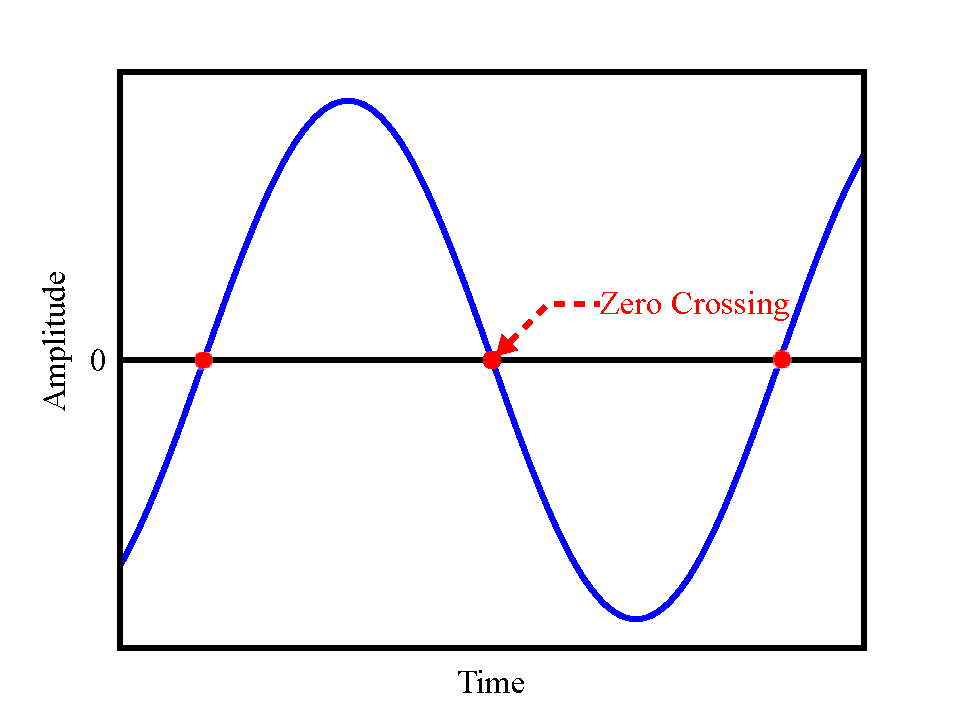
\includegraphics[width=3in]{ang/zero_crossing_illustration}
\caption{Zero Crossing Illustration (from Wikipedia)}
\label{zero_crossing_illustration}
\end{figure}

As is illustrated in Fig. \ref{zero_crossing_illustration}, a zero-crossing is a point where the \textbf{sign} of a signal changes, represented by a crossing of the time axis where amplitude is zero in the graph. Zero-crossing count is the times of zero-crossing occurrence in a stipulated period. Zero-crossing count of the $j$-th frame can be mathematically represented in (\ref{eq:frame-zcc}).

\begin{equation}
\label{eq:frame-zcc}
Z_s[j] = \sum_{n=1}^{N-1} \Big| \sgn(s_j[n]) - \sgn(s_j[n+1]) \Big|
\end{equation}
\begin{equation}
\sgn(s_j[n]) =
\begin{cases}
1, &s_j[n] \ge 0\\
0, &s_j[n] < 0
\end{cases}
\end{equation}

%--------------------------------------------

\subsection{Features of Different Frame Types}

We manually identify the unvoiced region and voiced region (the remains are silent region) of several different words by hearing the sound and observing the waveform.

\begin{figure}[H]
\begin{minipage}[t]{0.5\linewidth}
\centering
\minipageplot{ang/threshold_example1}
\caption{Waveform, $E_s$ \& $Z_s$}
\label{threshold_example1}
\end{minipage}
\begin{minipage}[t]{0.5\linewidth}
\centering
\minipageplot{ang/threshold_example2}
\caption{Waveform, $E_s$ \& $Z_s$ (Zoomed-in)}
\label{threshold_example2}
\end{minipage}
\end{figure}

In the case of word \textit{zero}, Fig. \ref{threshold_example1} shows the waveform and corresponding frame energy as well as the zero-crossing count of each frame. Fig. \ref{threshold_example2} is a zoomed-in version of Fig. \ref{threshold_example1}. The \textcolor{green_html}{green} dash-dot rectangle stands for the unvoiced region while the \textcolor{red}{red} dashed rectangle indicates voiced region. We can clearly see that unvoiced frames have low energy but high zero-crossing count, voiced frames have high energy but low zero-crossing count while silent frames have not only low energy but also low zero-crossing count. The relationships are summarized in Table \ref{table:thresholds}.

\begin{table}[H]
\centering
\caption{Properties of Different Frame Types}
\label{table:thresholds}
\begin{tabu} to 0.8\textwidth {XXX}
\toprule
Type &Energy &Zero-crossing count\\
\hline
Voiced &high &low\\
\hline
Unvoiced &low &high\\
\hline
Silent &low &low\\
\bottomrule
\end{tabu}
\end{table}

%--------------------------------------------

\subsection{Find Thresholds}

Fig. \ref{threshold1} shows the methods taken to find the energy threshold and the zero-crossing threshold. At the beginning, we manually identify the voiced and unvoiced frames of different words. Then, we calculate the average energy of these voiced frames and take noise level into consideration, finally determine a frame energy threshold. Analogously, we calculate the mean zero-crossing count of unvoiced frames and take the noise frequency into account, eventually obtain the zero-crossing threshold.\\

Note that thresholds are subject to the change of recording devices and environment noise. Hence, they have to be calibrated after the system is implemented on the DSP board and integrated with the \textit{Least Mean Square} noise cancellation scheme.

\begin{figure}[H]
\centering
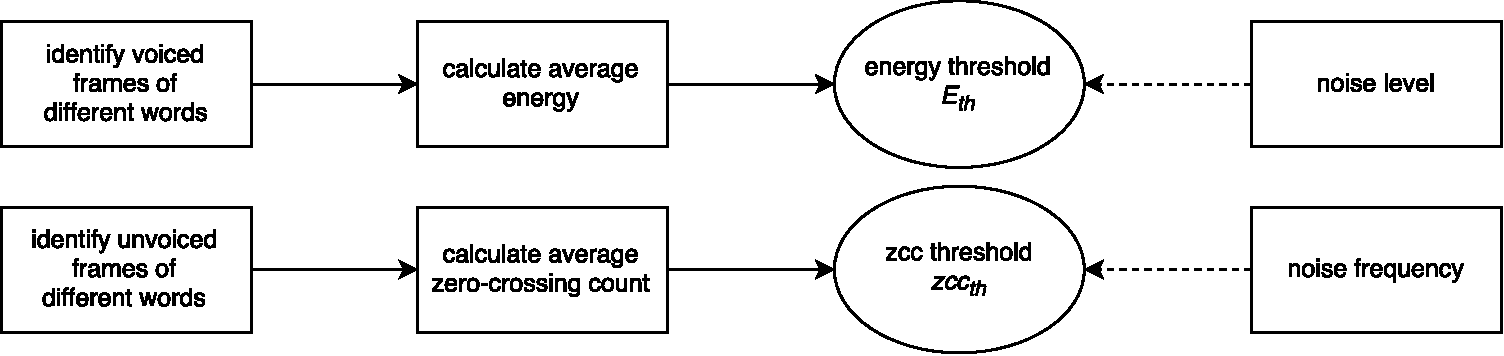
\includegraphics[width=5in]{ang/threshold1}
\caption{Methodology to Find Thresholds}
\label{threshold1}
\end{figure}

%--------------------------------------------

\subsection{Decision Rule}

Fig. \ref{threshold2} shows the decision-making strategy based on the thresholds obtained from above. Firstly, we calculate the energy of a frame and compare the energy with the threshold. A frame with higher energy is regarded as a voiced frame. Then, compute the zero-crossing count of low energy frame. If zero-crossing count is higher than the threshold, this frame is considered as unvoiced frame; otherwise, this frame will be discarded.

\begin{figure}[H]
\centering
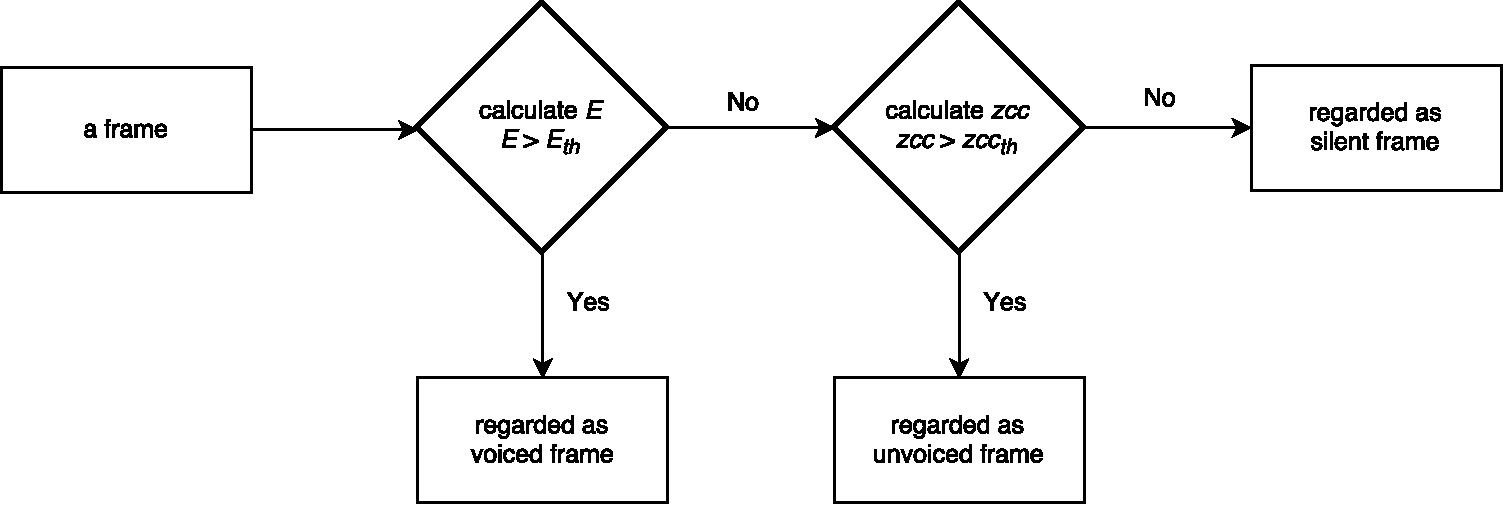
\includegraphics[width=5in]{ang/threshold2}
\caption{Decision Rule}
\label{threshold2}
\end{figure}

%--------------------------------------------
%--------------------------------------------

\section{Mel-frequency Cepstral Coefficients Extraction}
\label{subsection:mfcc}

Once informative frames are picked out by discarding the silent frames, the next stage is to calculate the Mel-frequency cepstral coefficients for each frame. MFCC algorithm is based on the concept of power cepstrum. The whole process to obtain power cepstrum defined in (\ref{eq:time-domain-to-cepstrum}) on page \pageref{eq:time-domain-to-cepstrum} can be divided into three procedures.
\begin{enumerate}
	\item Compute the Discrete Fourier Transform $S_j[k]$ and corresponding power spectrum $\hat{S}_j[k]$ of a time-domain signal $s_j[n]$.
	\item Take the logarithm of the power spectrum $\hat{S}_j[k]$.
	\item Conduct inverse Fourier transform.
\end{enumerate}

From previous section, we have known human hearing responds to the entire critical band instead of individual frequencies in this band. Thus, MFCC calculates the total power within each certain mel-scale band prior to log scaling (step 2). Moreover, MFCC substitutes Discrete Cosine Transform for inverse Fourier transform to reduce the computational complexity.

\subsection{Power Spectrum}

Discrete Fourier Transform (\ref{eq:dft}) constitutes the cornerstone of spectrum analysis.
\begin{equation}
\label{eq:dft}
S_j[k] = \sum_{n=1}^{N} s_j[n] W_N^{(n-1) k} \quad k = 1, 2, \dots, N
\end{equation}
\begin{equation}
W_N = e^{\frac{- 2\pi i}{N}}
\end{equation}

It can be clearly seen that the computations required by DFT increase dramatically as length $N$ increases. Due to the high computational requirement, direct implementation of DFT for large sequences has not been feasible. However, Fast Fourier Transform has made implementation of DFT practical in real-time processing.\\

FFT algorithms commonly implement a divide-and-conquer approach, i.e. an $N$-point DFT is successively divided into smaller DFTs. One of the most popular FFT algorithms is Radix-2 which restricts the sample length to a power of two. Therefore, we chose the frame length $N = 512$ (the 9th power of 2) to make full use of the FFT function. Table \ref{table:radix-2} compares the computational requirements of DFT and Radix-2 based FFT.

\begin{table}[H]
\caption{Computational Requirements of DFT and Radix-2 FFT}
\label{table:radix-2}
\begin{tabu} to \textwidth {X[c]X[c]X[c]}
\toprule
&$N$ &$N = 512$\\
\hline
DFT multiplications &$N^2$ &262144\\
\hline
DFT additions &$N^2 - N$ &261632\\
\hline
FFT multiplications &$\frac{N}{2} \log_2(N)$ &2304\\
\hline
FFT additions &$N \log_2(N)$ &4608\\
\bottomrule
\end{tabu}
\end{table}

We have known that the DFT $X[k]$ of a real sequence $x[n]$ is a conjugate symmetric sequence (from ELEN90058 \textit{Signal Processing} Workshop 3), i.e.
\begin{equation}
X[k] = X^*[\langle-k\rangle_{N}] = X^*[N-k]
\end{equation}

When computing the power spectrum, we are motivated to use this symmetry property and discard the last $(\frac{N}{2} - 1)$ points. Specifically, $S_j[1]$ is DC component of the signal; $S_j[2]$ to $S_j[\frac{N}{2}]$ are the first half of the complex spectrum; $S_j[\frac{N}{2} + 1]$ is the component at Nyquist frequency (8000 Hz).
\begin{equation}
\label{eq:power-spectrum}
\hat{S}_j[k] = |S_j(k)|^2 \quad k = 1, 2, \dots, \frac{N}{2} + 1
\end{equation}

%--------------------------------------------

\subsection{Bank Filtering}

The energy within each mel-scale bank can be computed by (\ref{eq:mel-filter}).
\begin{equation}
\label{eq:mel-filter}
X_j[m] = \sum^{\frac{N}{2} + 1}_{k=1} \hat{S}_j[k] H_{mel}[m, k] \quad m = 1, 2, \dots, M
\end{equation}
where $H_{mel}[m, k]$ is the gain of the $k$-th power spectrum data point within bank $m$.\\

\begin{equation}
\label{eq:mel-bank-gain}
H_{mel}[m, k] =
\begin{cases}
0 &f_{d2c}(k) \le f[m-1]\\
\displaystyle\frac{k - f[m-1]}{f[m] - f[m-1]} &f[m-1] < f_{d2c}(k) \le f[m]\\
\displaystyle\frac{f[m+1] - k}{f[m+1] - f[m]} &f[m] < f_{d2c}(k) \le f[m+1]\\
0 &f_{d2c}(k) > f[m+1]
\end{cases}
\end{equation}
where $f_{d2c}(k) = (k-1) \cdot \frac{F_s}{N}$ transforming the index $k$ of DFT into continuous-time frequency.

$f[m]$ ($m = 0, 1, \dots, M+1$) are equally spaced in mel-scale and can be computed by (\ref{eq:bank-boundary}).
\begin{equation}
\label{eq:bank-boundary}
f[m] = \mel^{-1} \left( \mel(f_{\min}) + m \cdot \frac{\mel(f_{\max}) - \mel(f_{\min})}{M + 1} \right)
\end{equation}
where the mel-scale to frequency transform $\mel^{-1}(m_{mel})$ is the inverse function of (\ref{eq:mel-function}).
\begin{equation}
\label{eq:mel-function-inverse}
f = \mel^{-1}(m_{mel}) = 700 \left( 10^{\left(\frac{m_{mel}}{2595}\right)} - 1 \right); \quad f \text{ in Hz}
\end{equation}

We take $f_{\min}$ = 0 Hz and $f_{\max} = \frac{F_s}{2}$ = 8000 Hz as per the system specification and $M = 20$ according to \cite{davis1980comparison}. $f[m]$ in Hz and corresponding mel-scale are listed in the appendix on page \pageref{table:frequency-mel-relationship}.

\begin{figure}[H]
\centering
\wideplot{ang/mel_triangle}
\caption{Mel Filter Banks}
\label{mel_triangle}
\end{figure}

Fig. \ref{mel_triangle} shows that $H_{mel}$ given in (\ref{eq:mel-bank-gain}) and (\ref{eq:bank-boundary}) is essentially a band-pass filter for each bank. $H_{mel}$ offers maximal gain 1 at $f[m]$ (the `central frequency' of bank $m$ in mel-scale) and then linearly decreases to 0 until reaching adjacent frequency boundaries ($f[m-1]$ and $f[m+1]$) on both sides.

%--------------------------------------------

\subsection{Log Scaling}

\begin{equation}
\label{eq:log-scaling}
\hat{X}_j[m] = \log_{10}(X_j[m]) \quad m = 1, 2, \dots, M
\end{equation}

%--------------------------------------------

\subsection{Discrete Cosine Transform}

\begin{equation}
\label{eq:dct}
\hat{C}_j[n] = \sqrt{\frac{2}{M}} \sum^{M}_{m=1} \hat{X}_j[m] \cos \left( \frac{\pi}{M} (m - 0.5) (n-1) \right) \quad n = 1, 2, \dots, F
\end{equation}
